\documentclass{beamer}
\usepackage{amsmath,amsthm}
\usepackage{amssymb}
\usepackage[english]{babel}
\usepackage{latexsym}
\usepackage{amsfonts}
\usepackage{graphicx}
\usepackage{float}
\usepackage{graphics}
\usepackage{epsfig}
\usepackage{url}
\usepackage{tikz}
% \usetheme{Madrid}
\usetheme{Boadilla}
% \usecolortheme{Boadilla}
\usepackage{multirow}

\DeclareMathOperator{\modulus}{mod}

\mode<presentation>

\title{Renormalization and rigidity}

\author{Joseph Adams}
\date{June 6, 2022}

\begin{document}
\begin{frame}

\titlepage

\end{frame}

\begin{frame}
    \frametitle{Overview}
    \tableofcontents
\end{frame}

\begin{frame}{The big picture}
\begin{itemize}
    \item Define renormalization of quadratic dynamical systems
    \item Give sufficient conditions for the existence of \emph{a priori} bounds
    \item Prove that these conditions imply combinatorial rigidity
    \item To non-mathematicians: Sorry... This is a math talk.
    \item To mathematicians: Sorry... I'll skip all the details.
\end{itemize}
\end{frame}

\section{Background}
\begin{frame}{Complex numbers}

\begin{definition}
A \emph{complex number} has the form $a+bi$, where $a$ and $b$ are real numbers, and $i=\sqrt{-1}$. $\mathbb{C}$ denotes the set of all complex numbers.
\end{definition}

\begin{itemize}
    \item Addition: $(a+bi)+(c+di)=(a+c)+(b+d)i$
    \item Multiplication: $(a+bi)\cdot(c+di)=(ac-bd)+(ad+bc)i$
    \item We can visualize the complex numbers as a 2-dimensional plane.
\end{itemize}

% \begin{itemize}
% \item First Sentence.
% \item<2-> ``Appears''
% \item<2->  Appears. Brueckner(2000)
% \end{itemize}
\end{frame}

\begin{frame}{Complex functions}
    \begin{itemize}
        \item Elementary calculus considers functions $f:\mathbb{R}\rightarrow\mathbb{R}$.
        \item Elementary calculus generalizes to functions $f:\mathbb{C}\rightarrow\mathbb{C}$.
        \item A differentiable complex function $f$ has a derivative $f'$. Zeros of the derivative are \emph{critical points}
        \item Complex functions can be iterated: $f^2(z)=f(f(z))$. The \emph{$n$-th iterate} of $f$ is $f^n(z)=\underbrace{f(...(f}_{n\text{ times}}(z))$.
    \end{itemize}
    \begin{example}
        A \emph{complex quadratic} has the form $f(z)=z^2+c$, where $c$ is a complex number.
        \begin{itemize}
            \item $f'(z)=2z$, so $0$ is the critical point.
            \item $f^2(z)=(z^2+c)^2+c$.
        \end{itemize}
    \end{example}
\end{frame}

\section{Dynamics}

\begin{frame}{The Fatou set}
Consider a complex quadratic $f_c(z)=z^2+c$.
\begin{definition}
The \emph{Fatou set} $K_c$ of $f_c$ is the set of $z$ such that $f_c^n(z)\not\rightarrow\infty$ as $n\rightarrow\infty$.
\end{definition}
\begin{definition}
The \emph{Julia set} is the boundary of $K_c$.
\end{definition}
For historical reasons, we'll sometimes call $K_c$ the Julia set.
\end{frame}

\begin{frame}{The Julia set can be connected}
\centering
$c=-0.1226+0.7449i$

\includegraphics[scale=0.25]{k_rabbit.png}
\end{frame}

\begin{frame}{The Julia set can be disconnected}
\centering
$c=-0.781+0.234j$

\includegraphics[scale=0.25]{k_cantor.png}
\end{frame}

\begin{frame}{Parameter space for quadratic dynamics}
\begin{theorem}[The fundamental dichotomy]
$K_c$ is either connected or totally disconnected.
\end{theorem}
\begin{theorem}
$K_c$ is connected if and only if $f_c^n(0)\not\rightarrow\infty$.
\end{theorem}
\begin{definition}
The \emph{Mandelbrot set} $M$ is the set of $c$ such that $K_c$ is connected.
\end{definition}
\end{frame}

\begin{frame}{The Mandelbrot set}
\centering
\includegraphics[scale=0.25]{m_default.png}

Can you see the little copies of the Mandelbrot set?
\end{frame}

\section{Little copies}

\begin{frame}{Period 3: Little copy}
\centering
$c=-1.754877666246693$

\includegraphics[scale=0.2]{m_p3.png}
\includegraphics[scale=0.2]{m_default.png}
\end{frame}

\begin{frame}{Period 3: Julia set}
\centering
$c=-1.754877666246693$

\includegraphics[scale=0.25]{k_p3.png}
\end{frame}

\begin{frame}{Period 4: Little copy}
\centering
$c=-0.156520166833755+1.032247108922832i$

\includegraphics[scale=0.2]{m_default.png}
\includegraphics[scale=0.2]{m_p4.png}
\end{frame}

\begin{frame}{Period 4: Julia set}
\centering
$c=-0.156520166833755+1.032247108922832i$

\includegraphics[scale=0.25]{k_p4.png}
\end{frame}

\begin{frame}{Are there little-little copies?}

{\bf Observations}
\begin{itemize}
    \item Little copies look like the Mandelbrot set.
    \item We've seen little copies for periods 3 and 4.
\end{itemize}
{\bf Question}

Is there a little-little copy in the period 4 little copy corresponding to the period 3 little copy in the Mandelbrot set?
\end{frame}

\begin{frame}{Period 12: Little copy}
\centering
$c=-0.167349208205021+1.041178661132973i$

\includegraphics[scale=0.2]{m_p12.png}
\includegraphics[scale=0.2]{m_p4.png}
\end{frame}

\begin{frame}{The period 12 LC corresponds to the period 3 LC}
\centering
\begin{tabular}{c c c}
    \begin{tabular}{c}\includegraphics[scale=0.12]{m_p12.png}\end{tabular} &
    \begin{tabular}{c}is to\end{tabular} &
    \begin{tabular}{c}\includegraphics[scale=0.12]{m_p4.png}\end{tabular}
    \\
    & as &
    \\
    \begin{tabular}{c}\includegraphics[scale=0.12]{m_p3.png}\end{tabular} &
    \begin{tabular}{c}is to\end{tabular} &
    \begin{tabular}{c}\includegraphics[scale=0.12]{m_default.png}\end{tabular}
\end{tabular}
\end{frame}

\begin{frame}{Period 12: Julia set}
\centering
$c=-0.167349208205021+1.041178661132973i$

\includegraphics[scale=0.25]{k_p12.png}

It looks like a little period 3 Julia set is embedded in the period 4 Julia set.
\end{frame}

\section{Renormalization}

\begin{frame}{Renormalization 1: Zoom in to the little Julia set}
\centering
Zoom in to the center of the period 12 Julia set.

\includegraphics[scale=0.2]{k_p12.png}
\includegraphics[scale=0.2]{k_p12_zoom.png}
\end{frame}

\begin{frame}{Renormalization 2: Straighten out the little Julia set}
\centering
\includegraphics[scale=0.2]{k_p12_zoom.png}
\includegraphics[scale=0.2]{k_p3.png}

We obtain the period 3 Julia set.
\end{frame}

\begin{frame}{Combinatorial model: Forget about the little Julia set}
\centering
Blur your eyes so that each little period 3 Julia set just looks like a blob.

\includegraphics[scale=0.2]{k_p12.png}
\includegraphics[scale=0.2]{k_p4.png}

We obtain the period 4 Julia set.
\end{frame}

\begin{frame}{Renormalization: A vague definition}
Let $f$ be a \emph{renormalizable} quadratic.
\begin{definition}
The \emph{renormalization} $Rf$ of $f$ is the quadratic obtained by zooming in to a little embedded Julia set.
\end{definition}
The renormalization scheme we'll discuss is called \emph{primitive} renormalization in mathematical literature.
\begin{definition}
The \emph{combinatorial model} $Hf$ of $f$ is the shape/dynamics of the big Julia set, where we forget about what happens on the little Julia sets.
\end{definition}
We can think of $Hf$ as the quadratic obtained by replacing each little Julia set with a blob/disk. In mathematical literature, the combinatorial model coincides with the \emph{Hubbard tree}.
\end{frame}

\begin{frame}{Renormalization: Definition via example}
\begin{center}
    \includegraphics[scale=0.1]{k_p12.png}
    \hspace{5pt}
    \includegraphics[scale=0.2]{p12_schematic.png}
    \hspace{5pt}
    \includegraphics[scale=0.1]{k_p3.png}
\end{center}
\begin{enumerate}
    \item Draw a small, topological disk $U$ around the central little Julia set.
    \item Iterate $U$ until it returns to the central little Julia set. Let $V=f^4(U)$ denote the topological disk so obtained.
    \item The central little Julia set is the set of points that never escape $U$ under iterates of $Rf=f^4$.
    \item $Rf=f^4:U\rightarrow V$ is a period 4 renormalization of $f$.
    \item  $Rf$ is \emph{quadratic-like} and equivalent to the quadratic associated with the period 3 Julia set.
\end{enumerate}
\end{frame}

\section{\textit{A priori} bounds and rigidity}

\begin{frame}{Quadratic-like maps}

\only<1>{
\begin{definition}A \emph{quadratic-like} map is a degree $2$ branched cover $f:U\rightarrow V$, where
\begin{itemize}
    \item $U$ and $V$ are topological disks,
    \item $\overline{U}\subset V$, and
    \item the Fatou set, $K=\bigcap_{n=1}^\infty f^{-n}(U)$, is connected.
\end{itemize}
The \emph{modulus} of $f$, denoted $\modulus f$, is the conformal thickness of the annulus $V\setminus\overline{U}$.
\end{definition}
\begin{center}
    \begin{tabular}{c c}
        \begin{tabular}{c}
            \includegraphics[scale=0.5]{ql.png}
        \end{tabular}
        &
        \parbox{5cm}{
            \begin{align*}
                U &= \text{light blue disk} \\
                V &= \text{dark blue disk} \\
                f &= \text{black arrow}\\
                K &= \text{black continuum within }U
            \end{align*}
        }
    \end{tabular}
\end{center}
}

\only<2>{
\begin{itemize}
    \item A quadratic-like map is equivalent, i.e., hybrid conjugate, to a quadratic.
    \item A renormalization of a quadatic or quadratic-like map is a quadratic-like map.
\end{itemize}
\begin{example}
Let $f(z)=z^2+c$ have a connected Julia set. The restriction of $f$ to a small disk around its Julia set is a quadratic-like map.
\end{example}
}
\end{frame}

\begin{frame}{Canonical renormalization leads to improvement of life}
Let $f:U\rightarrow V$ be a quadratic-like renormalization. There's too much freedom in choosing $U$ and $V$.
\begin{definition}
If $U$ and $V$ are chosen so that they maximize $\modulus f$, then we call $f$ a \textit{canonical} renormalization.
\end{definition}

\begin{theorem}[Improvement of life]
There exists a threshold $\mu>0$, depending only on certain combinatorial data, such that if $Rf$ is a canonical renormalization of $f$, then \[\modulus Rf<\mu \Rightarrow \modulus f < \mu/2.\]
\end{theorem}
% This theorem was proven by Jeremy Kahn for unicritical polynomial-like maps. I generalized this theorem to polynomial-like maps with more than one critical point.
\end{frame}

\begin{frame}{Infinite renormalization}
\begin{definition}
Suppose that a quadratic $f$ admits infinitely many renormalizations \[f_n=f^{p_n}:(U_n, K_n)\rightarrow (V_n, K_n)\] around its critical point.
\begin{itemize}
    \item $f$ is \textit{infinitely renormalizable}.
    \item $f$ has \emph{bounded combinatorics} if $p_{n+1}/p_n\leq B<\infty$ for all $n$.
    \item $f$ has \emph{a priori bounds} if $\modulus f_n\geq \mu>0$ for all $n$.
\end{itemize}
\end{definition}
From now on, we'll assume that the renormalizations $f_n$ are canonical.
\end{frame}

\begin{frame}{Beau bounds}

\only<1>{
\begin{center}
    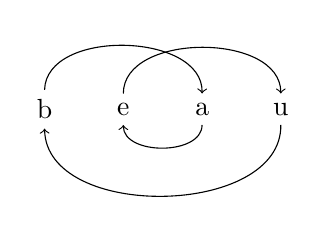
\begin{tikzpicture}
    \node (b) at (0, 0) {b};
    \node (e) at (1, 0) {e};
    \node (a) at (2, 0) {a};
    \node (u) at (3, 0) {u};
    \draw[->, bend left=90]
    (b) edge (a)
    (a) edge (e)
    (e) edge (u)
    (u) edge (b);
    \end{tikzpicture}

    beau = bounded and eventually universally bounded
\end{center}
}
\pause

\begin{theorem}[Beau bounds]
Let $B>0$. There exists $\mu>0$, depending only on $B$, such that if $f$ is an infinitely renormalizable quadratic with combinatorics bounded by $B$, then \[\modulus f_n\geq \mu>0\] for large enough $n$.
\end{theorem}
In fact, $\modulus f_n\geq\mu$ for all $n\geq N$, where $N$ depends only on $B$ and $\modulus f$.
\begin{theorem}[\textit{A priori} bounds]
If $f$ is an infinitely renormalizable quadratic with bounded combinatorics, then $f$ has \textit{a priori} bounds.
\end{theorem}
\end{frame}

\begin{frame}{Rigidity}
\begin{theorem}[Rigidity]
Let $f$ and $g$ be infinitely renormalizable quadratics with bounded combinatorics. Assume that the combinatorial models of $f_n$ and $g_n$ coincide for each $n$. Then $f=g$.
\end{theorem}
\end{frame}

\begin{frame}{Proof of rigidity}

\only<1>{
Consider a renormalization $f_n$.
\begin{center}
    \includegraphics[scale=0.1]{p12_schematic.png}
\end{center}
The dynamical picture gives rise to the domain $S_n$, drawn in orange.
\begin{center}
    \includegraphics[scale=0.1]{s_domain.png}
\end{center}
}

\only<2>{
The existence of \textit{a priori} bounds implies that the $S_n$ domains and the annular domains $A_n$ (between $S_n$ and $S_{n+1}$) have bounded geometry.
\begin{center}
    \includegraphics[scale=0.1]{t_domain.png}
\end{center}
Bounded combinatorics and the upper bound on the thickness of the annular domains $A_n$ ensures that the amount of twist across any $A_n$ is bounded.
}

\only<3>{
\begin{enumerate}
\item Coincidence of the combinatorial models implies that $f$ and $g$ are topologically equivalent.
\item Bounded geometry and bounded twists, together with Sullivan's pullback argument, allow us to promote the topological equivalence to quasiconformal equivalence.
\item Inou's invariant line theorem allows us to promote the quasiconformal equivalence to hybrid equivalence.
\item Hybrid equivalence here implies conformal equivalence.
\end{enumerate}
}
\end{frame}

% \begin{frame}{Motivation}
% \begin{enumerate}
%     \item Understanding quadratic dynamics amounts to understanding the Mandelbrot set.
%     \item The Mandelbrot set is well-understood, except for parameters $c$ where the corresponding quadratic $f_c$ admits infinitely many renormalizations.
%     \item For these $c$, the goal is to prove the existence of \textit{a priori} bounds.
% \end{enumerate}
% \end{frame}

\end{document}
